\documentclass[UTF8]{ctexart}
\author{李昂, 李逸翔, 李雪卉}
\title{基于 TensorFlow 与 Keras 卷积神经网络的猫类图像识别}
\usepackage{amsmath}
\usepackage{amssymb}
\usepackage{url}
\usepackage{geometry}
\usepackage{appendix}
\usepackage{booktabs}
\usepackage{cases}
\usepackage{graphicx}
\usepackage{subfigure}
\usepackage{listings}
\usepackage{xcolor}
\usepackage{fancyhdr}

\pagestyle{fancy}
\lhead{}
\rhead{}
\chead{}
\lfoot{}
\cfoot{\thepage}
\rfoot{}
\renewcommand{\headrulewidth}{0pt}
\renewcommand{\footrulewidth}{0pt}

\linespread{1.5}
\geometry{left=2.5cm,right=2.5cm,top=2.5cm,bottom=2.5cm}
\bibliographystyle{gbt7714-2005}

\begin{document}
\maketitle
\begin{abstract}
随着人工智能、机器学习技术的快速发展,这些新名词正在逐渐进入大众的视野当中。其中,图像识别、图像分类技术作为计算机视觉(Computer Vision)技术构成的重要环节,在人工智能发展中占据重要的位置。
本文通过给定数据集中 209 张猫类图片进行监督学习,通过 4 层卷积(Convolution)、池化(Pooling)与 2 层前馈层(Feed-Forward Layer)进行学习,其中卷积层分别根据 $64 \times 64 \times 3$ 的图像进行卷积,依次达到 32 层、64 层、128 层、256 层,之后进入有 512 个神经元的前馈层,并使用 ReLU 作为卷积层激活函数(Activate Function)、Sigmoid 作为最终输出神经元的激活函数。最终检验测试集,该模型准确率达到 90.0\%。
\begin{flushleft}
\textbf{关键词:} 卷积神经网络; 深度学习; 图像识别
\end{flushleft}
\end{abstract}

\clearpage

\section{题目重述}
给定一个已经标记有 “猫” 和 “非猫” 的训练数据集(Training Dataset)以及一个结构类似的测试数据集(Testing Dataset),建立一个简单的图像识别模型来准确地将猫的图片与其他的图片进行分类。每个图像都具有固定宽度与长度、以 RGB 值来表示每个像素。

\section{符号说明}
\begin{table}[htbp]
\centering
\caption{符号说明}
\label{signs}
\begin{tabular*}{0.8\textwidth}{p{100pt} | p{200pt}}
\hline
符号               & 相关说明       \\ \hline
$\omega$         & 路径权值       \\
$A_m$            & 图像矩阵       \\
$B$              & 卷积核矩阵      \\
$C$              & 输出层矩阵      \\
$\mathcal{A, B}$ & 池化(线性变换过程) \\
$K$              & 2 层前馈神经元矩阵 \\ \hline
\end{tabular*}
\end{table}

\section{基本假设}
\begin{enumerate}
\item 不考虑图像的旋转、缩放等任意变换;
\item 不考虑在完全相同的图像中选取。
\end{enumerate}

\section{问题分析}
所给题目共分为问题陈述(Problem Statement)、已知数据(datasets)、相关图片(images)三部分。由问题陈述可知,本题为图像识别类问题,目的是将一系列已知图片区分为 “猫” 和 “非猫” 两类;由相关图片分析可知,本题所需数学模型应具有根据猫的特征准确识别图片的功能;接下来将通过分析已知数据的特征来进行对模型的初步建立。

已知数据中包含训练数据集(train\_catvnoncat.h5)和测试数据集(test\_catvnoncat.h5)两部分。其中, train\_catvnoncat.h5 给出了三组数据,除 list\_classes 为介绍说明之外,其余两组分别为训练图像与标签。其中 train\_set\_x 是一个 $209 \times 64 \times 64 \times 3$ 的四维向量空间,即 209 个图像中,每个图像均为 $64 \times 64$ 像素,每个像素由一组 RGB 值(8-bit, 0-255)表示。以下为单个图像降维之后的向量表示样例:

而且 train\_catvnoncat.h5 之中每个图像(第一维度的 209 个)都有 label(train\_set\_y)与之一一对应。同理, test\_catvnoncat.h5 中的数据形式亦是如此。故根据如上的 train\_catvnoncat.h5 与 test\_catvnoncat.h5 中数据的特征,我们引入卷积神经网络来提取并学习图像的特征。

卷积神经网络是一种由人工神经网络发展而来的一种多层次网络结构,可以通过特征提取和特征映射过程进行快速训练,且识别准确率较高,因此常被应用于图像识别系统。卷积神经网络包含卷积层、池化层、全连接层等多种层次,可直接接收二维对象,经过多个阶段的卷积和抽样过程,将所提取到的特征输入到全连接层进行结果的计算,从而得到最终的识别结果。

\section{模型建立}
考虑到过于复杂的神经网络模型会导致时间开销过大,我们建立了两层卷积层(Convolution Layer,每层包含池化过程)、两层普通前馈层(Feed-Forward Layer)的神经网络,并定义卷积核为 $5 \times 5$ 大小,并使用 Python 语言与 TensorFlow、Keras 框架编写程序。

\begin{figure}[htbp]
  \centering
  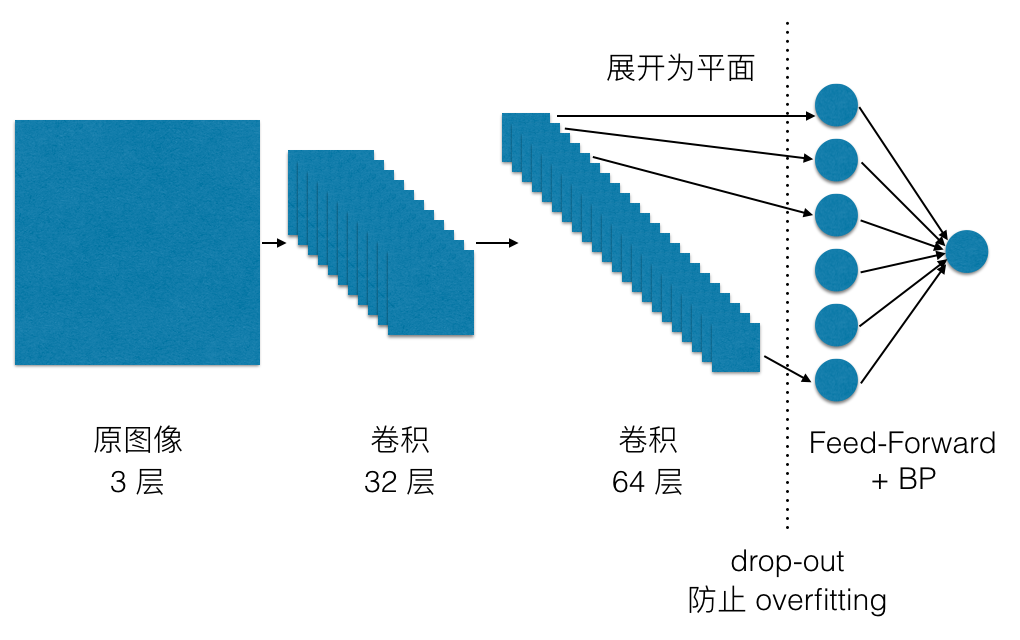
\includegraphics[width=0.95\textwidth]{../reference/convolution.png}
  \caption{模型的神经网络图}
  \label{fig:shapes0}
\end{figure}

其中第一层卷积层导出 32 层卷积核,作为提取的特征的一部分输入到池化 / 下一层卷积过程中。第二层卷积层导出 64 层卷积核,并通过 reshape 过程将两层卷积 / 池化导出的 $5 \times 5 \times 64$ 卷积核展开,导入之后的 4096 个前馈神经元,并通过 2 层前馈神经网络得到最终结果。

\subsection{卷积与池化}
对于两个参与卷积运算的矩阵
$$
A = 
\left[
\begin{matrix}
a_{11} & a_{12} & ... & a_{1m} \\
a_{21} & a_{22} & ... & a_{2m} \\
... & ... & ... & ... \\
a_{m1} & a_{m2} & ... & a_{mm}
\end{matrix}
\right]
, B = 
\left[
\begin{matrix}
b_{11} & b_{12} & ... & b_{1n} \\
b_{21} & b_{22} & ... & b_{2n} \\
... & ... & ... & ... \\
b_{n1} & b_{n2} & ... & b_{nn}
\end{matrix}
\right]
$$
(满足 $m > n$),将卷积核 $B$ 在二维平面上平移,并且卷积核的每个元素与被卷积图像对应位置相乘,再求和。
$$
A * B = 
\left[
\begin{matrix}
\sum_{i = m - n + 1}^{m}\sum_{j = m - n + 1}^{m}b_{ij}a_{i-n+1, j-n+1} & \sum_{i = m - n + 1}^{m}\sum_{j = m - n + 1}^{m}b_{ij}a_{i-n+1, j-n+2} & ... \\ % & \sum_{i = m - n + 1}^{m}\sum_{j = m - n + 1}^{m}b_{ij}a_{i-n+1, j} \\
\sum_{i = m - n + 1}^{m}\sum_{j = m - n + 1}^{m}b_{ij}a_{i-n+2, j-n+1} & \sum_{i = m - n + 1}^{m}\sum_{j = m - n + 1}^{m}b_{ij}a_{i-n+2, j-n+2} & ...  \\ % & \sum_{i = m - n + 1}^{m}\sum_{j = m - n + 1}^{m}b_{ij}a_{i-n+2, j} \\
... & ... & ... \\
\sum_{i = m - n + 1}^{m}\sum_{j = m - n + 1}^{m}b_{ij}a_{i, j-n+1} & \sum_{i = m - n + 1}^{m}\sum_{j = m - n + 1}^{m}b_{ij}a_{i, j-n+2} & ... \\ % & \sum_{i = m - n + 1}^{m}\sum_{j = m - n + 1}^{m}b_{ij}a_{ij}
\end{matrix}
\right]
$$
卷积运算常见于计算机视觉、图像处理等方面,由于具备将图像信息压缩的能力,在深度学习、图像分类中常用于提取图像特征。但是,对于题目中 $64 \times 64$ 像素的 RGB 图像,若通过学习得到了 400 个压缩成 $32 \times 32$ 大小的图像特征,那么每一个图像特征与原图像卷积都会得到 $(64 - 32 + 1)^2$ 的图像特征,而且只是单个特征的计算量;并且庞大的运算容易失去控制而导致过拟合(overfitting)。所以我们引入池化(pooling)过程,对于不同位置的特征进行统计,降低特征维度,同时不影响卷积过程中产生的新的特征信息。

\subsection{前馈神经网络}
人工神经网络(Artificial Neural Network)发展自人类对于动物神经系统工作方式、学习与记忆方式的观察。科学家最早提出的神经网络模型被称为感知机(Perceptron),由多个输入数据 $a_1, a_2, ..., a_n$、对应多个权重值 $\omega_1, \omega_2, ..., \omega_n$、一个输出阈值 $t$ 与一个输出数据 $b$ 组成。
$$
b = 
\left\{
\begin{aligned}
1, \quad \omega \cdot a \geqslant t,\\
0, \quad \omega \cdot a < t
\end{aligned}
\right.
$$
$\omega$(权重)通过人工给定初始值,在遍历训练集的过程中,通过指定增减学习率(learning rate)、不断修正错误($b$ 导出值与实际不符)来调整 $\omega$。
更复杂的前馈神经网络具有 1 到 2 层的隐藏层(hidden layer),用于处理高维输入值、提高模型准确率,同时允许多个输出值。

同时,为了规避单一感知机的线性不可分问题,隐藏层、输出层的神经元在接受上一层输入后,会通过特定的激活函数(Activate Function)将线性的向量内积转化为非线性的空间划分。我们采用了 Sigmoid 函数
$$y = \frac{1}{1 + e^{\omega \cdot a}}$$
作为该神经元的输出。

在解决这一问题的过程中,我们采用了 2 层前馈网络。第一层为输入层(在整个网络中是隐藏层),接收上一层卷积 / 池化层输入的特征;第二层则为整个网络中最终的输出层,通过一个神经元输出最终的 0 和 1。

\begin{figure}[htbp]
  \centering
  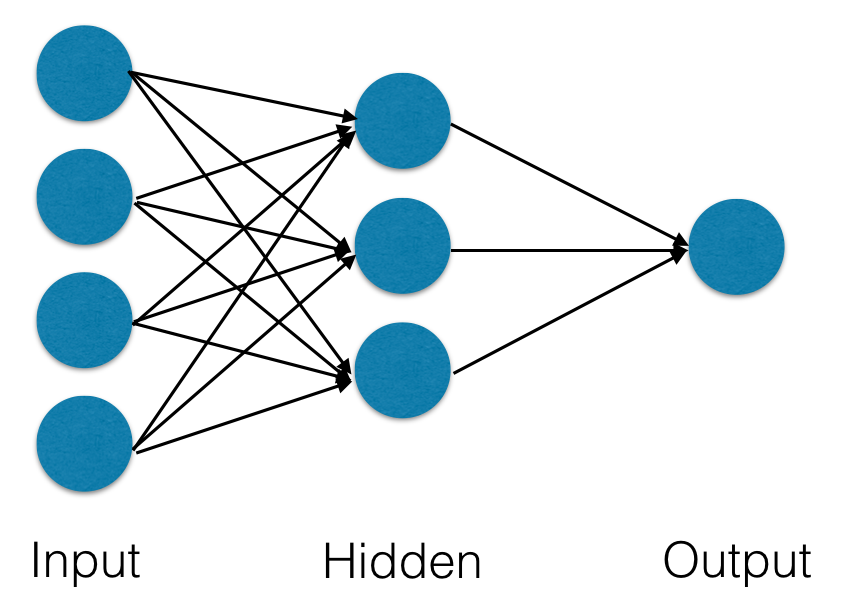
\includegraphics[width=0.95\textwidth]{../reference/feed-forward.png}
  \caption{前馈神经网络}
  \label{fig:shapes1}
\end{figure}

\section{模型求解}
随机初始化路径权值 $\omega = (\omega_1, ..., \omega_n)$,并且服从 $\mu = 0.2, \sigma = 0.1$ 的正态分布。
遍历训练数据集(train\_catvnoncat.h5 文件中的 train\_set\_x、train\_set\_y)部分。
对于单个图像 $A_m$,首先将其与预设置的 $5 \times 5$ 卷积核 $B$ 进行步长为 1 的卷积,得到该层输出
$$A * B = C^{(1,1)}_{62 \times 62}$$
,其中 $C$ 为该卷积层输出 32 层的其中一层;进入第一层池化进行最大池化方案(max-pooling):
$$\mathcal{A}^{(1)}(C^{(1,1)}_{62 \times 62}) = C^{(1,2)}_{32 \times 32}$$
第二层卷积 / 池化类似:
$$C^{(1,2)}_{32 \times 32} * B = C^{(2,1)}_{30 \times 30}$$
$$\mathcal{A}^{(2)}(C^{(2,1)}_{30 \times 30}) = C^{(2,2)}_{16 \times 16}$$
,其中 $C$ 为该卷积层输出 64 层中的其中一层。至此完成卷积、数据提取过程。

将 64 层 $C^{(2,2)}_{16 \times 16}$ 展开为一维向量
$$\mathcal{B}(64C^{(2,2)}_{16 \times 16}) = c^{(3)}_{16384 \times 1}$$
,其中 $16384 = 64 \times 16 \times 16$;并且使 $c^{(3)}$ 各维度 与 4096 个前馈神经元全连接。对于单个该层神经元 $K^{(1)}$ 则会产生输出
$$K^{(1)} = \frac{1}{1 + e^{\omega^{(3)} \cdot c^{(3)}}}$$
,最终输出层则为
$$K^{(2)} = \frac{1}{1 + e^{\omega^{(4)} \cdot K^{(1)}}}$$
。实际运行中,以上过程对于单一数据集进行了 40 次遍历,以在防止过拟合的情况下获得最佳结果。

\section{模型检验}
我们在以上计算机求解过程中,每次遍历完成后都会通过 test\_catvnoncat.h5 文件中的数据集检验一次运行情况。40 次的全部运行情况如图 3,其中最后一行输出(Out)分别为测试集的最终 loss 与 accuracy。

\begin{figure}[htbp]
  \centering
  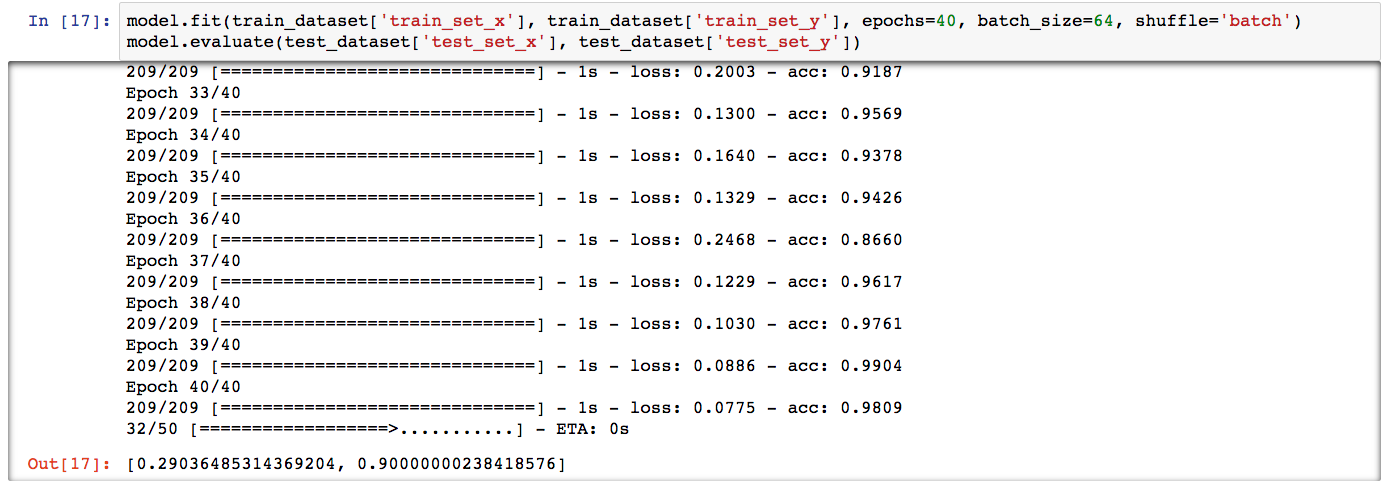
\includegraphics[width=0.95\textwidth]{../reference/result.png}
  \caption{最终结果}
  \label{fig:shapes2}
\end{figure}

\section{模型评价与推广}
\subsection{模型评价}
该方法基于卷积神经网络模型,采用两层卷积层、两层普通前馈层,其中卷积层采用了池化过程,对于不同位置的特征进行统计,降低特征维度,同时不影响卷积过程中产生的新
的特征信息,避免了庞大的运算造成失控导致的过拟合,具有较高的图像识别能力,经过检验可达到90.0\%的准确率。但是它只能处理规定格式的静态图像,具有一定的局限性。

\subsection{模型推广}
如今,人工智能在计算机领域占有越来越重要的地位,而图像识别技术正是人工智能中重要的一部分。此模型可模仿人脑中的神经网络,通过一定量的学习,可直接将输入的图像转化为图像识别结果进行输出。本文中所建立的卷积神经网络模型仅可用于区分图片中是否有 “猫” ,若经过推广,使该神经网络系统学习更多事物的特征,那么此模型将可识别越来越多的事物;若经过更深度的推广,此模型甚至可以识别各种事物甚至人物。最终可应用于对于一般图片的基本识别,实现了对人眼的解放,从而实现了进一步的人工智能。


\clearpage
\appendix
\appendixname
\section{程序源码}
带有运行结果的源码与部分互动界面可以通过 Jupyter Notebook 打开根文件夹中的 /code 文件夹内的 cat-recognition-2.ipynb 文件来查看。

以下代码均为 Python 语言(Python 3)。

\begin{lstlisting}[language=Python]
from PIL import Image
import h5py as h5
import numpy as np
import pandas as pd
import tensorflow as tf
import time
import tensorflow.contrib.keras as kr

train_dataset = h5.File('datasets/train_catvnoncat.h5')
Image.fromarray(train_dataset['train_set_x'][27])

test_dataset = h5.File('datasets/test_catvnoncat.h5')
Image.fromarray(test_dataset['test_set_x'][47])

from tensorflow.contrib.keras import layers, models, optimizers

model = models.Sequential()

model.add(layers.Convolution2D(
    batch_input_shape=(None, 64, 64, 3),
    filters=32,
    kernel_size=5,
    strides=1,
    padding='same',
    data_format='channels_first',
))
model.add(layers.Activation('relu'))
model.add(layers.MaxPooling2D(
    pool_size=2,
    strides=2,
    padding='same',
    data_format='channels_first',
))

model.add(layers.Convolution2D(16, 5, strides=1, padding='same',
        data_format='channels_first'))
model.add(layers.Activation('relu'))
model.add(layers.MaxPooling2D(2, 2, 'same', data_format='channels_first'))

model.add(layers.Convolution2D(32, 5, strides=1, padding='same', 
        data_format='channels_first'))
model.add(layers.Activation('relu'))
model.add(layers.MaxPooling2D(2, 2, 'same', data_format='channels_first'))

model.add(layers.Convolution2D(64, 5, strides=1, padding='same', 
        data_format='channels_first'))
model.add(layers.Activation('relu'))
model.add(layers.MaxPooling2D(2, 2, 'same', data_format='channels_first'))

model.add(layers.Convolution2D(128, 5, strides=1, padding='same', 
        data_format='channels_first'))
model.add(layers.Activation('relu'))
model.add(layers.MaxPooling2D(2, 2, 'same', data_format='channels_first'))

model.add(layers.Convolution2D(256, 5, strides=1, padding='same', 
        data_format='channels_first'))
model.add(layers.Activation('relu'))
model.add(layers.MaxPooling2D(2, 2, 'same', data_format='channels_first'))

model.add(layers.Flatten())
model.add(layers.Dense(512))
model.add(layers.Activation('relu'))

model.add(layers.Dense(1))
model.add(layers.Activation('sigmoid'))

adam = optimizers.Adam(lr=1e-4)
model.compile(optimizer=adam,
              loss='binary_crossentropy',
              metrics=['accuracy'])

model.fit(train_dataset['train_set_x'], train_dataset['train_set_y'], epochs=40, 
        batch_size=64, shuffle='batch')
model.evaluate(test_dataset['test_set_x'], test_dataset['test_set_y'])
\end{lstlisting}

\end{document}